\section{The Universe}

\epigraph{\emph{Talking, talking. Spinning a web of words, pale walls of dreams,
between myself and all I see.}} {---John Gardner, \emph{Grendel}}

You will now write your first \emph{abstract data type}, commonly referred to as
an \textbf{ADT}. This ADT will provide the abstraction for a universe, a
\emph{finite} 2-D grid of cells. Why not an infinite grid? Because computers
work in \emph{finite memory}. The following subsections will walk you through
the list of constructor, destructor, accessor, and manipulator functions
required for your ADT. You will be supplied \texttt{universe.h} (in the
Resources repository), the header file for the \texttt{Universe} ADT and you
\textcolor{red}{\textbf{may not}} modify it.

The universe will be abstracted as a \texttt{struct} called \texttt{Universe}.
We will use a \texttt{typedef} to construct a new type, which you should treat
as opaque --- which means that you must pretend that you cannot manipulate it
directly. \textbf{C}, unlike some more modern languages, \emph{does not enforce
opacity}.

Here, \texttt{universe.h} \emph{declares} the new type and \texttt{universe.c}
\emph{defines} its concrete implementation. Once again,
\textcolor{red}{\textbf{you cannot modify \texttt{universe.h.}}}

\begin{clisting}{}
struct Universe {
    uint32_t rows;
    uint32_t cols;
    bool **grid;
    bool toroidal;
};
\end{clisting}

An instance of a \texttt{Universe} must contain the following fields:
\texttt{rows}, \texttt{cols}, and a 2-D boolean grid, \texttt{grid}. Since there
are two states: \emph{alive} and \emph{dead}, then a natural choice for
representing the states is the \texttt{bool} type. A cell with the value
\texttt{false} in \texttt{grid} indicates that the cell is dead; the value
\texttt{true} indicates that the cell is alive. It is also possible for a
\texttt{Universe} to be \emph{toroidal}, which is indicated by the
\texttt{toroidal} field. \textcolor{red}{This \texttt{struct} definition must be
placed in the file \texttt{universe.c}.}

\begin{funcdoc}{\texttt{Universe *uv\_create(uint32\_t rows, uint32\_t cols, bool toroidal)}}
  This is the constructor function that creates a \texttt{Universe}. The first two
  parameters it accepts are the number of \texttt{rows} and \texttt{cols},
  indicating the dimensions of the underlying \emph{boolean} grid. The last
  parameter \texttt{toroidal} is a boolean. If the value of \texttt{toroidal} is
  \texttt{true}, then the universe is \emph{toroidal}. The \emph{return type} of
  this function is of type \texttt{Universe *}, meaning the function should return
  a \emph{pointer} to a \texttt{Universe}. You will be using the \texttt{calloc()}
  function from \texttt{<stdlib.h>} to dynamically allocate memory. For more
  information on \texttt{calloc()}, read \texttt{man calloc}. Here is an example
  of allocating a matrix of \texttt{uint32\_t}s:

\begin{clisting}{}
uint32_t **matrix = (uint32_t **) calloc(rows, sizeof(uint32_t *));
for (uint32_t r = 0; r < rows; r += 1) {
    matrix[r] = (uint32_t *) calloc(cols, sizeof(uint32_t));
}
\end{clisting}

  Note that we first allocate a column of pointers  to rows, and then we allocate
  the actual rows. For an example of a complete ADT constructor function, see the
  section on ADTs in the course coding standards.
\end{funcdoc}

\begin{funcdoc}{\texttt{void uv\_delete(Universe *u)}}
  This is the destructor function for a \texttt{Universe}. Simply put, it frees
  any memory allocated for a \texttt{Universe} by the constructor function.
  Unlike Java and Python, \textbf{C} is \emph{not} garbage collected. Not
  freeing allocated memory by the end a program results in a \emph{memory leak}.
  Your programs should be free of memory leaks. In the case of multilevel data
  structures such as a \texttt{Universe}, we must free the inside first. Imagine
  getting rid of a water bucket: you should dump out the water before scrapping
  the bucket. Use \texttt{valgrind} to check for memory leaks -- the graders
  will too!
\end{funcdoc}

\begin{funcdoc}{\texttt{uint32\_t uv\_rows(Universe *u)}}
  Since we will be using \texttt{typedef} to create \emph{opaque} data types, we
  need functions to access fields of a data type. These functions are called
  \emph{accessor} functions. An opaque data type means that users do not need to
  know its implementation outside of the implementation itself. This means that
  it is incorrect to have \texttt{u->rows} outside of \texttt{universe.c} as it
  violates opacity. This function returns the number of rows in the specified
  \texttt{Universe} (it is possible, but only inside \texttt{universe.c}).
\end{funcdoc}

\begin{funcdoc}{\texttt{uint32\_t uv\_cols(Universe *u)}}
  Like \texttt{uv\_rows()}, this function is an accessor function and returns
  the number of columns in the specified \texttt{Universe}.
\end{funcdoc}

\begin{funcdoc}{\texttt{void uv\_live\_cell(Universe *u, uint32\_t r, uint32\_t c)}}
  The need for \emph{manipulator} functions follows the rationale behind the need
  for accessor functions: we need some way to alter fields of a data type. This
  function simply marks the cell at row \texttt{r} and column \texttt{c} as live.
  If the specified row and column lie outside the bounds of the universe, nothing
  changes. Since we are using \emph{bool}, we assume that \emph{true} means live
  and \emph{false} means dead.
\end{funcdoc}

\begin{funcdoc}{\texttt{void uv\_dead\_cell(Universe *u, uint32\_t r, uint32\_t c)}}
  This function marks the cell at row \texttt{r} and column \texttt{c} as
  \emph{dead}. Like in \texttt{uv\_live\_cell()}, if the row and column are
  out-of-bounds, nothing is changed.
\end{funcdoc}

\begin{funcdoc}{\texttt{bool uv\_get\_cell(Universe *u, uint32\_t r, uint32\_t c)}}
  This function returns the value of the cell at row \texttt{r} and column
  \texttt{c}. If the row and column are out-of-bounds, \texttt{false} is
  returned. Again, \emph{true} means the cell is live.
\end{funcdoc}

\begin{funcdoc}{\texttt{bool uv\_populate(Universe *u, FILE *infile)}}
  This function will populate the \texttt{Universe} with row-column pairs read in
  from \texttt{infile}. This function will require the use of \texttt{<stdio.h>}
  since \texttt{infile} is a \texttt{FILE *} (\texttt{FILE} is defined in the
  \texttt{<stdio.h>} library). The necessary \emph{include} will be supplied in
  \texttt{universe.h} for you. A valid input file that could be fed into your
  program would be:

\begin{clisting}{}
36 65
2 32
3 30
\end{clisting}

  The first line of a valid input file for your program consists of the number
  of rows followed by the number of columns of the universe. Each subsequent
  line is the row and column of a live cell. You will want a loop that makes
  calls to \texttt{fscanf()} to read in all the row-column pairs in order to
  populate the universe. If a pair lies beyond the dimensions of the universe,
  and return \texttt{false} to indicate that the universe failed to be
  populated. Return \texttt{true} if the universe is successfully populated.
  Failure to populate the universe should cause the game to fail with an error
  message. \textcolor{red}{\emph{Do not} print in functions if you can avoid it
  -- unless that is their job!}
\end{funcdoc}

\begin{funcdoc}{\texttt{uint32\_t uv\_census(Universe *u, uint32\_t r, uint32\_t c)}}
  \begin{wrapfigure}{r}{0.125\textwidth}
    
\includegraphics[width=0.125\textwidth]{images/horns.jpg}
  \end{wrapfigure}

  When we consider our universe, a flat universe is simply a grid.  Ideally in
  the Game of Life, that extends to infinity in the $\pm x$ and $\pm y$
  directions. Since we cannot have an infinite grid, we are left with a choice:
  we can either, as the Flat Earthers believe, have things fall off the edge or
  come up with some other solution. Our solution will be to treat the finite
  grid as a flat Earth or as a \emph{torus}. An example of a torus can be
  constructed by taking a rectangular strip of flexible material, for example, a
  rubber sheet, and joining the top edge to the bottom edge, and the left edge
  to the right edge, without any half-twists.

  It requires some reflection, but if you think about you will see that a torus
  is any topological space that is topologically equivalent to a torus. A coffee
  cup and a doughnut are both topological tori.

  \begin{center}
    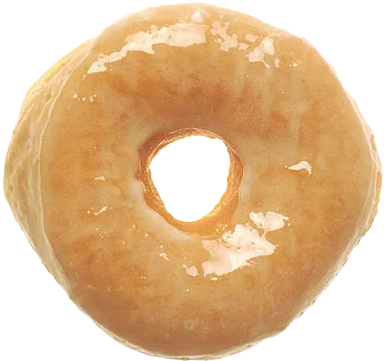
\includegraphics[width=1.7in]{images/donut.png}\hfil
    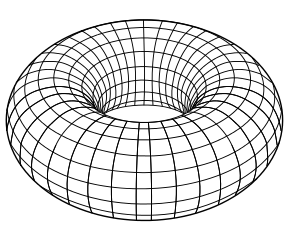
\includegraphics[width=2in]{images/torus.png}\hfil
    
\includegraphics[width=1.7in]{images/cup.png}
  \end{center}

  In the realm of real numbers, the parametric equation of a ring torus is:
\begin{align*}
x(\theta, \phi) &= (R + r \cos \theta) \cos \phi \\
y(\theta, \phi) &= (R + r \cos \theta) \sin \phi \\
z(\theta, \phi) &= r \sin \theta
\end{align*}

  \noindent where $\theta$, and $\phi$ are angles which make a full circle, so
  that their values start and end at the same point, $R$ is the distance from the
  center of the tube to the center of the torus, and $r$ is the radius of the
  tube.  Our torus is finite and discrete: in other words, assuming a square grid
  $G_{n,n}$ indexed from $0, \ldots, n-1$ (because we are Computer Scientists),
  the right edge of the grid $G_{i, n-1}$ is connected (succeeded by) $G_{i, 0}$,
  and the bottom edge of the grid $G_{n-1, i}$ is connected to $G_{0, i}$. In
  other words, \emph{successor} and \emph{predecessor} are calculated using
  \emph{modular arithmetic} if the universe is a torus, which you have seen these
  functions before.

  This function returns the number of \emph{live neighbors} adjacent to the cell
  at row \texttt{r} and column \texttt{c}. If the universe is flat, or
  non-toroidal, then you should only consider the \emph{valid} neighbors for the
  count. If the universe is toroidal, then all neighbors are valid: you simply
  wrap to the other side. \textcolor{red}{Tip: you should calculate the row and
  column for each neighbor and apply modular arithmetic if the universe is
  toroidal.}
\end{funcdoc}

\begin{funcdoc}{\texttt{void uv\_print(Universe *u, FILE *outfile)}}
  This functions prints out the universe to \texttt{outfile}. A live cell is
  indicated with the character `\texttt{o}' (a lowercase O) and a dead cell is
  indicated with the character `\texttt{.}' (a period). You will want to use
  either \texttt{fputc()} or \texttt{fprintf()} to print to the specified
  \texttt{outfile}. Since you cannot print a torus, you will always print out
  the flattened universe.
\end{funcdoc}
